% HEADLINE FIGURE: the strict language hierarchy regular ⊊ VPL ⊊ DCFL ⊆ CFL, with each
% CSM protocol placed in its band, and the closure/decidability annotations that make VPL
% the sweet spot. Palette: regular=indigo, VPL=violet, DCFL=slate, CFL=grey.
\documentclass[border=12pt]{standalone}
\usepackage{tikz}
\usepackage{amssymb}
\usepackage{xcolor}
\usetikzlibrary{positioning, fit, backgrounds}
\definecolor{reg}{HTML}{4F46E5}
\definecolor{vpl}{HTML}{7C3AED}
\definecolor{dcfl}{HTML}{475569}
\definecolor{cfl}{HTML}{6B7280}
\definecolor{ink}{HTML}{1E293B}
\begin{document}
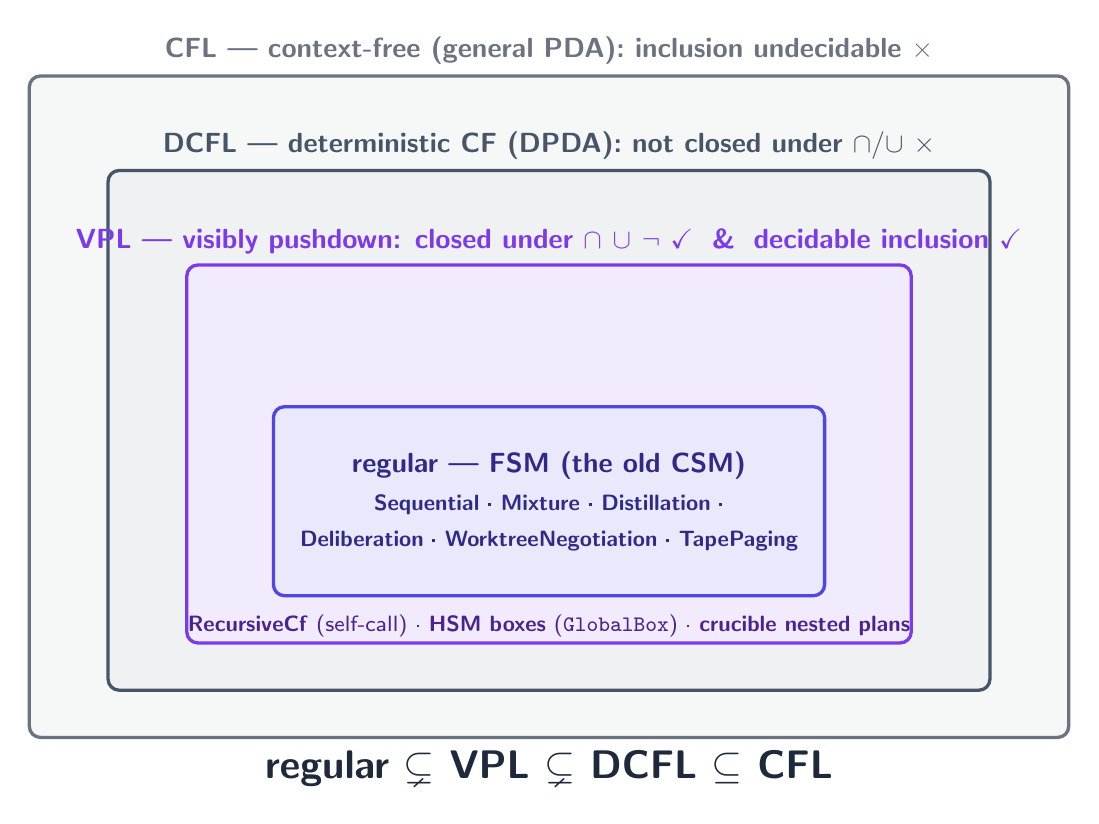
\begin{tikzpicture}[font=\sffamily]
  % Outer to inner concentric bands.
  \node[draw=cfl, very thick, rounded corners, fill=cfl!6, minimum width=132mm, minimum height=84mm,
        label={[text=cfl, font=\sffamily\bfseries]above:CFL — context-free (general PDA): inclusion \emph{undecidable} $\times$}] (cfl) {};
  \node[draw=dcfl, very thick, rounded corners, fill=dcfl!8, minimum width=112mm, minimum height=66mm,
        label={[text=dcfl, font=\sffamily\bfseries]above:DCFL — deterministic CF (DPDA): not closed under $\cap/\cup$ $\times$}] (dcfl) at (0,-3mm) {};
  \node[draw=vpl, very thick, rounded corners, fill=vpl!10, minimum width=92mm, minimum height=48mm,
        label={[text=vpl, font=\sffamily\bfseries]above:VPL — visibly pushdown: closed under $\cap\,\cup\,\neg$ $\checkmark$ \;\&\; decidable inclusion $\checkmark$}] (vpl) at (0,-6mm) {};
  \node[draw=reg, very thick, rounded corners, fill=reg!12, minimum width=70mm, minimum height=24mm] (reg) at (0,-12mm) {};

  % Regular-band contents.
  \node[text=reg!60!black, font=\sffamily\bfseries, align=center] at (reg) {regular — FSM (the \emph{old} CSM)\\[2pt]
    \footnotesize Sequential · Mixture · Distillation ·\\[1pt]\footnotesize Deliberation · WorktreeNegotiation · TapePaging};

  % VPL-band contents (between vpl and reg).
  \node[text=vpl!60!black, font=\sffamily\footnotesize, align=center, below=1mm of reg] {%
    \textbf{RecursiveCf} (self-call) · \textbf{HSM boxes} (\texttt{GlobalBox}) · \textbf{crucible nested plans}};

  % The strict-containment chain.
  \node[text=ink, font=\sffamily\Large\bfseries] at (0,-46mm) {regular $\subsetneq$ VPL $\subsetneq$ DCFL $\subseteq$ CFL};
\end{tikzpicture}
\end{document}
